\documentclass[convert = false, tikz]{standalone}
\usepackage[utf8]{inputenc}
\usepackage{tikz}
\usetikzlibrary{automata, positioning, arrows, calc, shapes.geometric}

\usepackage{../../../../style_automata}

% arara: pdflatex
% arara: latexmk: { clean: partial }
\begin{document}
\tikzset{
    node distance=1.25cm, % specifies the minimum distance between two nodes.
    }
    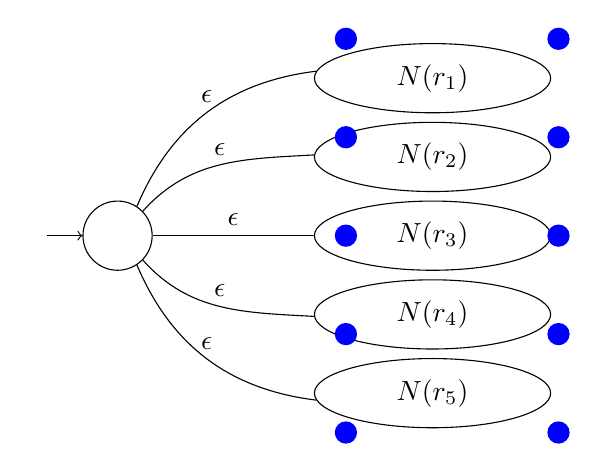
\begin{tikzpicture} 

        \node[state, initial, initial text=] (start) {};
        \node[state, ellipse, minimum width=3cm, right of=start, xshift=3cm] (r3) {$N(r_3)$};
        \node[state, ellipse, minimum width=3cm, above of=r3] (r2) {$N(r_2)$};
        \node[state, ellipse, minimum width=3cm, above of=r2] (r1) {$N(r_1)$};
        \node[state, ellipse, minimum width=3cm, below of=r3] (r4) {$N(r_4)$};
        \node[state, ellipse, minimum width=3cm, below of=r4] (r5) {$N(r_5)$};
        
        \draw
        (start) edge[above, bend left] node{$\epsilon$} (r1)
        (start) edge[above, bend left, in=165] node{$\epsilon$} (r2)
        (start) edge[above] node{$\epsilon$} (r3)
        (start) edge[above, bend right, in=195] node{$\epsilon$} (r4)
        (start) edge[above, bend right] node{$\epsilon$} (r5)
        ;

        \tikzset{every node/.style={circle,fill,inner sep=1mm,outer sep=1mm,color=blue}}
        \path
        (r1) to (2.90,2.5) node(dot11) {}
        (r1) to (5.60,2.5) node(dot12) {}
        (r2) to (2.90,1.25) node(dot21) {}
        (r2) to (5.60,1.25) node(dot22) {}
        (r3) to (2.90,0) node(dot31) {}
        (r3) to (5.60,0) node(dot32) {}
        (r4) to (2.90,-1.25) node(dot41) {}
        (r4) to (5.60,-1.25) node(dot42) {}
        (r5) to (2.90,-2.5) node(dot51) {}
        (r5) to (5.60,-2.5) node(dot52) {}
        ;
                
    \end{tikzpicture}
    \end{document}
    
    